\documentclass[11pt]{article}

\usepackage{times}
\usepackage{epsf}
\usepackage{epsfig}
\usepackage{amsmath, alltt, amssymb, xspace}
\usepackage{wrapfig}
\usepackage{fancyhdr}
\usepackage{url}
\usepackage{verbatim}
\usepackage{fancyvrb}
\usepackage{float}

\usepackage{subfigure}
\usepackage{cite}
\usepackage{hyperref}
\hypersetup{%
    pdfborder = {0 0 0}
}
\topmargin      -0.50in  % distance to headers
\oddsidemargin  0.0in
\evensidemargin 0.0in
\textwidth      6.5in
\textheight     8.9in


%\centerfigcaptionstrue

%\def\baselinestretch{0.95}


\newcommand\discuss[1]{\{\textbf{Discuss:} \textit{#1}\}}
%\newcommand\todo[1]{\vspace{0.1in}\{\textbf{Todo:} \textit{#1}\}\vspace{0.1in}}
\newtheorem{problem}{Problem}[section]
%\newtheorem{theorem}{Theorem}
%\newtheorem{fact}{Fact}
\newtheorem{define}{Definition}[section]
%\newtheorem{analysis}{Analysis}
\newcommand\vspacenoindent{\vspace{0.1in} \noindent}

%\newenvironment{proof}{\noindent {\bf Proof}.}{\hspace*{\fill}~\mbox{\rule[0pt]{1.3ex}{1.3ex}}}
%\newcommand\todo[1]{\vspace{0.1in}\{\textbf{Todo:} \textit{#1}\}\vspace{0.1in}}

%\newcommand\reducespace{\vspace{-0.1in}}
% reduce the space between lines
%\def\baselinestretch{0.95}

\newcommand{\fixmefn}[1]{ \footnote{\sf\ \ \fbox{FIXME} #1} }
\newcommand{\todo}[1]{
\vspace{0.1in}
\fbox{\parbox{6in}{TODO: #1}}
\vspace{0.1in}
}

\newcommand{\mybox}[1]{
\vspace{0.2in}
\noindent
\fbox{\parbox{6.5in}{#1}}
\vspace{0.1in}
}


\newcounter{question}
\setcounter{question}{1}

\newcommand{\myquestion} {{\vspace{0.1in} \noindent \bf Question \arabic{question}:} \addtocounter{question}{1} \,}

\newcommand{\myproblem} {{\noindent \bf Problem \arabic{question}:} \addtocounter{question}{1} \,}



\newcommand{\copyrightnotice}[1]{
\vspace{0.1in}
\fbox{\parbox{6in}{
			This lab was developed by Sparta Global for Cybersecurity courses.
			It was built based on the original lab that was developed for the Labtainer framework by the Naval Postgraduate School, Center for Cybersecurity and Cyber Operations under National Science Foundation Award No. 1438893.
      This work is in the public domain, and cannot be copyrighted.
			}}
\vspace{0.1in}
}


\newcommand{\idea}[1]{
\vspace{0.1in}
{\sf IDEA:\ \ \fbox{\parbox{5in}{#1}}}
\vspace{0.1in}
}

\newcommand{\questionblock}[1]{
\vspace{0.1in}
\fbox{\parbox{6in}{#1}}
\vspace{0.1in}
}


\newcommand{\argmax}[1]{
\begin{minipage}[t]{1.25cm}\parskip-1ex\begin{center}
argmax
#1
\end{center}\end{minipage}
\;
}

\newcommand{\bm}{\boldmath}
\newcommand  {\bx}    {\mbox{\boldmath $x$}}
\newcommand  {\by}    {\mbox{\boldmath $y$}}
\newcommand  {\br}    {\mbox{\boldmath $r$}}


\newcommand{\tstamp}{\today}
%\rfoot[\fancyplain{\tstamp} {\tstamp}]  {\fancyplain{}{}}

\pagestyle{fancy}
\lhead{\bfseries Labtainers}
\chead{}
\rhead{\small \thepage}
\lfoot{\small{\textit{Dr. Osama Abu Oun - Cybersecurity Courses - Sparta Global (\url{https://www.spartaglobal.com/})}}}
\cfoot{}
\rfoot{}

\begin{document}

\begin{center}
{\LARGE Routing Basics - Lab Guide}
\vspace{0.1in}\\
\end{center}

\copyrightnotice

\section{Overview}
This lab covers IP configuration and basic routing functionality used in Linux OS.

These include use of:
\begin{itemize}
	\item Add/Remove IP address using \texttt{ip address} command
	\item Add/Remove routes using \texttt{ip route} command
	\item Testing the connectivity using \texttt{ping} command
\end{itemize}

\section{Lab Environment}
This lab runs in the Labtainer framework,
available at http://my.nps.edu/web/c3o/labtainers.
That site includes links to a pre-built virtual machine
that has Labtainers installed, however Labtainers can
be run on any Linux host that supports Docker containers.

From your labtainer-student (~/labtainer/labtainer-student) directory start the lab using:
\begin{verbatim}
    labtainer sparta-routing-basics
\end{verbatim}
\noindent A link to this lab guide will be displayed.

\section{Network Configuration}
This lab includes several IP networks as in Figure~\ref{fig:topology}.
When the lab starts, you will get four virtual terminals, one connected to each component (Host/Router).
\newline
\newline
\textbf{\textit{IP addresses and routing are not configured}}
\newline
\newline
\textbf{Question 1:}
How many IP networks in the shown topology ?
\newline
\newline
\textbf{Question 2:}
Can you make enumerate these IP networks (Network IDs, Subnet Masks) ?
\newline
\newline

\begin{figure}[H]
\begin{center}
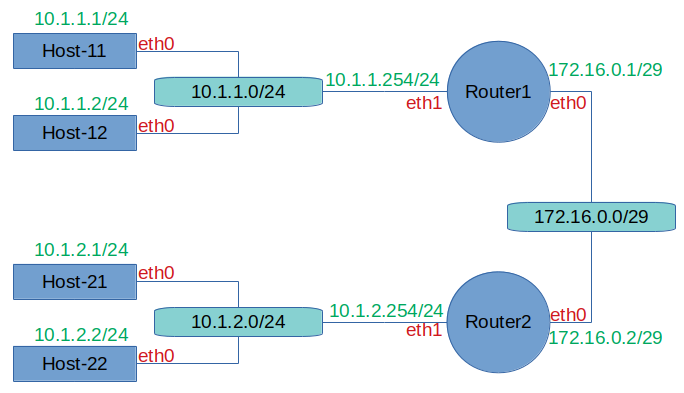
\includegraphics [width=0.8\textwidth]{labtainers-routing-basics-lab-01.png}
\end{center}
\caption{Network topology for routing-basics lab}
\label{fig:topology}
\end{figure}

\section{Credentials}
\begin{itemize}
	\item \textbf{Host-11}:
	\begin{itemize}
		\item \textbf{Username:} user-11
		\item \textbf{Password:} user-11
	\end{itemize}
	\item \textbf{Host-12}:
	\begin{itemize}
		\item \textbf{Username:} user-12
		\item \textbf{Password:} user-12
	\end{itemize}o
	\item \textbf{Host-21}:
	\begin{itemize}
		\item \textbf{Username:} user-21
		\item \textbf{Password:} user-21
	\end{itemize}
	\item \textbf{Host-22}:
	\begin{itemize}
		\item \textbf{Username:} user-22
		\item \textbf{Password:} user-22
	\end{itemize}o
	\item \textbf{Router1}:
	\begin{itemize}
		\item \textbf{Username:} admin
		\item \textbf{Password:} admin
	\end{itemize}
\end{itemize}

\section{Lab Tasks}
\subsection{Configuring Network 10.1.1.0/24}

\subsubsection{Host-11 Configuration}
Lets start by configuring the IP address and verify it
\textbf{IP address}: 10.1.1.1/24

\begin{verbatim}
    sudo ip address add 10.1.1.1/24 dev eth0
    ip address
\end{verbatim}

\textbf{Configuring the Default Gateway}: 10.1.1.254/24
\begin{verbatim}
    sudo ip route add default via 10.1.1.254
    ip route
\end{verbatim}

\subsubsection{Host-12 Configuration}
Lets start by configuring the IP address and verify it
\newline
\newline
\textbf{IP address}: 10.1.1.2/24

\begin{verbatim}
    sudo ip address add 10.1.1.1/24 dev eth0
    ip address
\end{verbatim}

\textbf{Configuring the Default Gateway}: 10.1.1.254/24

\begin{verbatim}
    sudo ip route add default via 10.1.1.254
    ip route
\end{verbatim}

\subsubsection{Testing the connectivity}
Lets make sure that the two hosts can exchange traffic.
\newline
\begin{itemize}
	\item On Host-11 (Ping Host-11 -$>$ Host-12)
	\begin{verbatim}
	    ping 10.1.1.2
	\end{verbatim}

	What is the result ?
	\item On Host-12 (Ping Host-12 -$>$ Host-11)
	\begin{verbatim}
	    ping 10.1.1.1
	\end{verbatim}

	What is the result ?
	\item On Host-11 (Ping Host-11 -$>$ Router1)
	\begin{verbatim}
	    ping 10.1.1.254
	\end{verbatim}

	What is the result ?
	\item On Host-12 (Ping Host-12 -$>$ Router1)
	\begin{verbatim}
	    ping 10.1.1.254
	\end{verbatim}

	What is the result ?
\end{itemize}


\subsubsection{Router1 Configuration}
Lets configure the IP address on eth1
\textbf{IP address}: 10.1.1.254/24

\begin{verbatim}
    sudo ip address add 10.1.1.254/24 dev eth1
    ip address
\end{verbatim}

\subsubsection{Testing the connectivity}
Lets make sure that the two hosts can exchange traffic.
\newline
\begin{itemize}
	\item On Host-12 (Ping Router1 -$>$ Host-11)
	\begin{verbatim}
	    ping 10.1.1.1
	\end{verbatim}

	What is the result ?
	\item On Host-11 (Ping Router1 -$>$ Host-12)
	\begin{verbatim}
	    ping 10.1.1.2
	\end{verbatim}

	What is the result ?
	\item On Host-11 (Ping Host-11 -$>$ Router1)
	\begin{verbatim}
	    ping 10.1.1.254
	\end{verbatim}

	What is the result ?
	\item On Host-12 (Ping Host-12 -$>$ Router1)
	\begin{verbatim}
	    ping 10.1.1.254
	\end{verbatim}

	What is the result ?
\end{itemize}


\subsection{Configuring Network 10.1.2.0/24}

\subsubsection{Host-21 Configuration}
Lets start by configuring the IP address and verify it
\newline
\newline
\textbf{IP address}: 10.1.2.1/24

\begin{verbatim}
    sudo ip address add 10.1.2.1/24 dev eth0
    ip address
\end{verbatim}

\textbf{Configuring the Default Gateway}: 10.1.2.254/24
\begin{verbatim}
    sudo ip route add default via 10.1.2.254
    ip route
\end{verbatim}

\subsubsection{Host-22 Configuration}
Lets start by configuring the IP address and verify it
\textbf{IP address}: 10.1.2.2/24

\begin{verbatim}
    sudo ip address add 10.1.2.1/24 dev eth0
    ip address
\end{verbatim}

\textbf{Configuring the Default Gateway}: 10.1.2.254/24

\begin{verbatim}
    sudo ip route add default via 10.1.2.254
    ip route
\end{verbatim}

\subsubsection{Testing the connectivity}
Lets make sure that the two hosts can exchange traffic.
\newline
\begin{itemize}
	\item On Host-21 (Ping Host-21 -$>$ Host-22)
	\begin{verbatim}
	    ping 10.1.2.2
	\end{verbatim}

	What is the result ?
	\item On Host-22 (Ping Host-22 -$>$ Host-21)
	\begin{verbatim}
	    ping 10.1.2.1
	\end{verbatim}

	What is the result ?
	\item On Host-21 (Ping Host-21 -$>$ Router2)
	\begin{verbatim}
	    ping 10.1.2.254
	\end{verbatim}

	What is the result ?
	\item On Host-22 (Ping Host-22 -$>$ Router2)
	\begin{verbatim}
	    ping 10.1.2.254
	\end{verbatim}

	What is the result ?
\end{itemize}


\subsubsection{Router2 Configuration}
Lets configure the IP address on eth1
\textbf{IP address}: 10.1.2.254/24

\begin{verbatim}
    sudo ip address add 10.1.2.254/24 dev eth1
    ip address
\end{verbatim}

\subsubsection{Testing the connectivity}
Lets make sure that the two hosts can exchange traffic.
\newline
\begin{itemize}
	\item On Host-22 (Ping Router2 -$>$ Host-21)
	\begin{verbatim}
	    ping 10.1.2.1
	\end{verbatim}

	What is the result ?
	\item On Host-21 (Ping Router2 -$>$ Host-22)
	\begin{verbatim}
	    ping 10.1.2.2
	\end{verbatim}

	What is the result ?
	\item On Host-21 (Ping Host-21 -$>$ Router2)
	\begin{verbatim}
	    ping 10.1.2.254
	\end{verbatim}

	What is the result ?
	\item On Host-22 (Ping Host-22 -$>$ Router2)
	\begin{verbatim}
	    ping 10.1.2.254
	\end{verbatim}

	What is the result ?
\end{itemize}

\subsection{Configuring Network 172.16.0.0/29}

\subsubsection{Router1 Configuration}
Lets start by configuring the IP address and verify it
\textbf{IP address}: 172.16.0.1/29

\begin{verbatim}
    sudo ip address add 172.16.0.1/29 dev eth0
    ip address
\end{verbatim}

\subsubsection{Router2 Configuration}
Lets start by configuring the IP address and verify it
\textbf{IP address}: 172.16.0.2/29

\begin{verbatim}
    sudo ip address add 172.16.0.1/29 dev eth0
    ip address
\end{verbatim}

\subsubsection{Testing the connectivity}
Lets make sure that the two routers can exchange traffic. Then lets try to check if the hosts on different networks can exchange any traffic
\newline
\begin{itemize}
	\item On Router1 (Ping Router1 -$>$ Router2:172.16.0.2)
	\begin{verbatim}
	    ping 172.16.0.2
	\end{verbatim}

	What is the result ?
	\item On Router2 (Ping Router2 -$>$ Router1:172.16.0.1)
	\begin{verbatim}
	    ping 172.16.0.1
	\end{verbatim}

	What is the result ?
	\item On Host-11 (Ping Host-11 -$>$ Host-21)
	\begin{verbatim}
	    ping 10.1.2.1
	    traceroute 10.1.2.1
	\end{verbatim}

	\item On Host-11 (Ping Host-11 -$>$ Host-22)
	\begin{verbatim}
	    ping 10.1.2.2
	    traceroute 10.1.2.2
	\end{verbatim}

	\item On Host-12 (Ping Host-12 -$>$ Host-21)
	\begin{verbatim}
	    ping 10.1.2.1
	    traceroute 10.1.2.1
	\end{verbatim}

	\item On Host-12 (Ping Host-12 -$>$ Host-22)
	\begin{verbatim}
	    ping 10.1.2.2
	    traceroute 10.1.2.2
	\end{verbatim}

	What is the result ?
\end{itemize}


\subsubsection{Routing Configuration: Router1}
Lets configure the routing on Router1
\textbf{Routing to 10.1.2.0/24: via 172.16.0.2}

\begin{verbatim}
    sudo ip route add 10.1.2.0/24 via 172.16.0.2
    ip route
\end{verbatim}

\subsubsection{Routing Configuration: Router2}
Lets configure the routing on Router2
\newline
\newline
\textbf{Routing to 10.1.1.0/24: via 172.16.0.1}

\begin{verbatim}
    sudo ip route add 10.1.1.0/24 via 172.16.0.1
    ip route
\end{verbatim}

\subsubsection{Testing the connectivity}
Lets make sure that all hosts can exchange traffic.
\newline
\begin{itemize}
	\item On Host-11 (Ping Host-11 -$>$ Host-21)
	\begin{verbatim}
	    ping 10.1.2.1
	    traceroute 10.1.2.1
	\end{verbatim}

	\item On Host-11 (Ping Host-11 -$>$ Host-22)
	\begin{verbatim}
	    ping 10.1.2.2
	    traceroute 10.1.2.2
	\end{verbatim}

	\item On Host-12 (Ping Host-12 -$>$ Host-21)
	\begin{verbatim}
	    ping 10.1.2.1
	    traceroute 10.1.2.1
	\end{verbatim}

	\item On Host-12 (Ping Host-12 -$>$ Host-22)
	\begin{verbatim}
	    ping 10.1.2.2
	    traceroute 10.1.2.2
	\end{verbatim}

	What is the result ?
\end{itemize}

\section{Submission}
After finishing the lab, go to the terminal on your Linux system that was used to start the lab and type:
\begin{verbatim}
    stoplab sparta-routing-basics
\end{verbatim}
When you stop the lab, the system will display a path to the zipped lab results on your Linux system.  Provide that file to
your instructor, e.g., via the Sakai site.

\end{document}
